\documentclass[12pt,twoside,onecolumn,openany]{book}

\usepackage{lmodern}
\usepackage[T1]{fontenc}
\usepackage[spanish,activeacute]{babel}
\decimalpoint %Cambiamos de comas a puntos en las ecuaciones
\usepackage[utf8]{inputenc} %Nos permite incluir los acentos de forma cotidiana
\usepackage{mathtools}%Permite ingresar los metodos matemáticos
\usepackage{listings}%Permite ingresar código fuente
\usepackage{fancyhdr}%Permite modificar el encabezado y pie de página
\usepackage{hyperref}%Nos permite crear links en el documento()
\usepackage[dvipsnames]{xcolor} %Nos permite definir colores
\usepackage{colortbl}% Permite darle color a las tablas
\usepackage{amsmath}% Se ocupa para poder escribir matrices
\setlength\headheight{30pt}% se agrega mas espacio al encabezado
\usepackage{subcaption}% permite juntar 2 imagenes en una misma linea
\usepackage{float}% obliga a las figuras a quedarse en su pocisión
\usepackage{tikzsymbols} %Permite agregar emoticones
\usepackage{enumerate} 
\usepackage{geometry} % permite editar los margenes del documento
%-----------Eliminamos la identación de los párrafos-------%
\setlength{\parindent}{0pt}


%-------- Se define las lineas del pie y encabezado de de página
\fancypagestyle{plain}{


   % \fancyfoot[L]{\begin{picture}(0,0) \put(0,-75){ 
\includegraphics[scale=0.7]{Imagenes/Foot-blue.png}}\end{picture}}

  %-------------Imagen de pie de página impares---------%
    \fancyfoot[L]{\begin{picture}(0,0) \put(-145,-65){ 
\includegraphics[scale=0.7]{Imagenes/Foot-blue.png}}\end{picture}}
	
  \renewcommand{\headrulewidth}{0.5pt}
  \renewcommand{\footrulewidth}{0.5pt}	
}

\pagestyle{plain}% aplicamos el estilo para todas las páginas


%------------------Definimos los colores a usar----------------%
\definecolor{myBlue}{HTML}{166995}
\definecolor{myDarkBlue}{HTML}{0D547B}
\definecolor{myGinda}{HTML}{921010}
\definecolor{myBlueRef}{HTML}{0277bd}
\definecolor{myBlueChapter}{HTML}{004784}
\definecolor{myWhite}{rgb}{250,250,250}


%---------Definimos el color de cada vínculo en el documento como links, urls, citas, etc.
\hypersetup{
    colorlinks=true,
    linkcolor=myBlueRef,
    filecolor=magenta,      
    urlcolor=myBlue,
    citecolor=myBlueRef,
    pdftitle={Sharelatex Example}
}



\begin{document}

  \begin{titlepage}

  \thispagestyle{empty}


  \begin{minipage}{.2\textwidth}
    \flushleft
%----------------------Logo IPN ---------------------------%
    \center{
\includegraphics[scale=.19]{imagenes/ipn.pdf}}


%----------------imagenLineasGuia---------------------------%    
    \vspace{20pt}

    \center{
      \rule{.5pt}{.6\textheight}
      \hspace{7pt}
      \rule{2pt}{.6\textheight}
      \hspace{7pt}
      \rule{.5pt}{.6\textheight}
    }
%----------------------Logo ESCOM ----------------------------%
    \center{
\includegraphics[scale=.07]{imagenes/logoescom.png}} 

  \end{minipage}
  \begin{minipage}{.8\textwidth}
  %---------------InfoTesis-------------------------%
    \flushright

    \center{

      \center{
        \LARGE{I}\large{NSTITUTO} \LARGE{P}\large{OLITÉCNICO} 
        \LARGE{N}\large{ACIONAL}
      } \\

      \rule{\textwidth}{1pt}\\
      \hrulefill\\[1cm]



      \LARGE{E}\large{SCUELA} \LARGE{S}\large{UPERIOR} \large{DE} \LARGE{C}\large{ÓMPUTO}\\[1cm]

      \large{ TRABAJO TERMINAL} \\[1cm]

      \textbf{ \LARGE{R}\LARGE{ecolector} \LARGE{y} \LARGE{clasificador} \LARGE{de}  
      \LARGE{noticias}}\\[1cm]
      \large{\textbf{2018-B013}}\\[1cm]


      \large{\textbf{PRESENTAN:}}\\[1cm]
      \large{CARLOS ANDRES HERNANDEZ GOMEZ}\\
      \large{LUIS DANIEL MEZA MARTÍNEZ}\\[1cm]


      \large{\textbf{DIRECTORES:  }}\\[.5cm]
      \large{\textbf{Dr.} JOEL OMAR JUÁREZ GAMBINO }\\
      \large{\textbf{Dra.} CONSUELO VARINIA GARCÍA MENDOZA }\\[0.5cm]

     \ \\
     Ciudad de México,\today

    }


  \end{minipage}
  \end{titlepage}

  

%Manual de Usuario
\section{Instalación}

	El presente sistema web ha sido desarrollado bajo el sistema operativo \textit{Ubuntu} en su versión 18.04.3, las siguientes bibliotecas serán instaladas utilizando la terminal del sistema operativo, son necesarias para el correcto funcionamiento del sistema
	\subsection{Recolector}
	El recolector ha sido construido bajo el lenguaje de programación \textit{Python} utilizando el framework \textit{Scrapy} el cual se utiliza para recuperar información de diversos sitios, para su instalación se utiliza el siguiente comando:
	\begin{lstlisting}[language=bash]
  		$ pip3 install Scrapy
	\end{lstlisting}

	\subsection{Clasificador}
	El clasificador ha sido programado bajo el lenguaje de programación \textit{Python}, previó a llevar a cabo el proceso de clasificación, se procede a realizar dos tareas importantes, tokenizar y lematizar; para realizar estas tareas se ha utilizado la biblioteca \textit{Spacy}, para su instalación se utiliza el comando:
	\begin{lstlisting}[language=bash]
  		$ pip3 install -U spacy
  		$ python -m spacy download es_core_news_sm
	\end{lstlisting}

	Para el clasificador se ha utilizado la biblioteca \textit{Scikit Learn}, para su instalación se utiliza el siguiente comando:
	\begin{lstlisting}[language=bash]
		$ pip3 install -U scikit-learn
	\end{lstlisting}

	\subsection{Aplicación Web}
	La presente aplicación Web ha sido desarrollada bajo el lenguaje de programación \textit{Java} es necesario instalar NetBeans en su versión 8.2, en la siguiente liga \textit{https://netbeans.org/downloads/8.2/} se encuentra la versión 8.2, debido a que se realiza una aplicación web es necesario instalar la versión \textit{Java EE} la cual incluye \textit{Apache TomCat}.
	\\
	Una vez que se ha descargado NetBeans nos ubicamos en la carpeta donde se haya descargado nuestro archivo y ejecutamos el siguiente comando:
	\begin{lstlisting}[language=bash]
		$ chmod +x netbeans-8.2-javaee-linux.sh 
		$ -/netbeans-8.2-javaee-linux.sh 
	\end{lstlisting}

	Una vez instaladas todas las bibliotecas previas, es necesario ubicarnos en la siguiente carpeta:
	\begin{lstlisting}[language=bash]
		/ApplicacionWeb/TT2/web/resources/Recolector$
	\end{lstlisting}
	Una vez ubicados en dicha carpeta ejecutaremos el siguiente comando:
	\begin{lstlisting}[language=bash]
		$ scrapy startproject TT2
	\end{lstlisting}
	
\section{Ejecución}
Una vez finalizada la instalación y creación del recolector, se procederá a abrir NetBeans, una vez ingresado se procederá a abrir el proyecto, como se muestra en la Figura \ref{fig:seleccionarProyecto}
\begin{figure}[H]
	\centering
	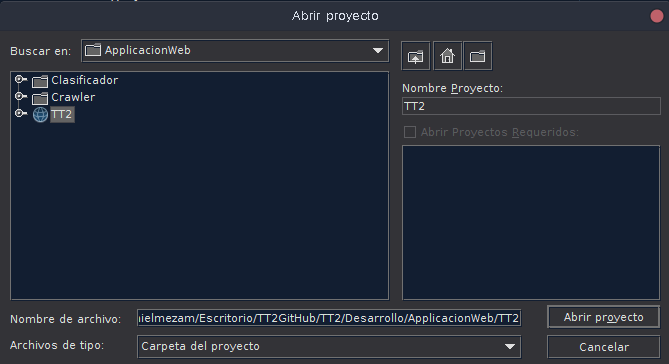
\includegraphics[scale=0.6]{imagenes/abrirProyecto.png}
	\caption{Se selecciona el proyecto TT2}
	\label{fig:seleccionarProyecto}
\end{figure}

Una vez abierto el proyecto se ejecutará el sistema, dando click derecho sobre el archivo \textit{inicio.xhtml} y seleccionando la opción ejecutar, el archivo se muestra en la Figura \ref{fig:inicio}

\begin{figure}[H]
	\centering
	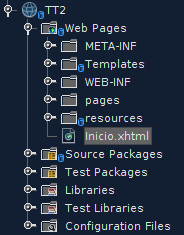
\includegraphics[scale=0.6]{imagenes/ejecutar.png}
	\caption{Se ejecuta el archivo inicio.xhtml}
	\label{fig:inicio}
\end{figure}


La aplicación esta diseñada en 4 etapas, las cuales son mostradas en la Figura \ref{fig:procesoAppWeb}, donde la etapa \textbf{Selección} describe las secciones disponibles para obtener noticias; la etapa \textbf{Recolectar} muestra la integración de los \textit{crawlers} en la herramienta; la etapa \textbf{Clasificar} hace uso del modelo clasificador desarrollado en la sección anterior y para concluir, la etapa \textbf{Mostrar resultados} describe la forma en que los datos son presentados al usuario. Es importante mencionar que las etapas en color azul cielo siempre son ejecutadas, sin embargo las de color gris no siempre son llevadas acabo. A continuación se explica a detalle cada una las tareas.


\begin{figure}[H]
	\centering
	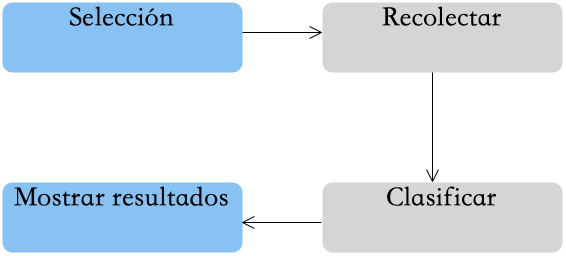
\includegraphics[scale=0.6]{imagenes/ProcesoAplicacionWeb.png}
	\caption{Etapas de la aplicación web}
	\label{fig:procesoAppWeb}
\end{figure}


\subsection{Selección}


Esta etapa permite elegir al usuario la sección de noticias a buscar. La aplicación comienza en una pantalla inicial, donde se muestra un menú con las opciones \textbf{Inicio}, \textbf{Cultura}, \textbf{Deportes}, \textbf{Economía}, \textbf{Política}, \textbf{Ciencia y Tecnología}, estas categorías (excluyendo \textbf{Inicio}) son las secciones permitidas para recolectar noticias, como se muestra en el Figura \ref{fig:PantallaInicio}. Cabe mencionar que la opción \textbf{Inicio}, permite regresar a la pantalla principal.\\


\begin{figure}[H]
\centering

\includegraphics[scale=0.35]{imagenes/pantallaPrincipal.png}
\caption{Pantalla de Inicio}
\label{fig:PantallaInicio}
\end{figure}

Después de elegir una sección, se muestra el mensaje \textbf{En proceso de recolección y clasificación}, como se visualiza en la Figura \ref{fig:loading}, el cual informa que las etapas \textbf{Recolectar} y \textbf{Clasificar} están en proceso, además cuando se muestra este mensaje no se puede seleccionar otra secciones hasta que el proceso haya concluido. Cabe destacar que el proceso continúa de forma normal si se cumplen las siguientes condiciones:

\begin{enumerate}
	\item \textbf{Primera vez}: Esta condición hace referencia a la etapa \textbf{selección}, es decir cuando es la primera vez que se ha selecciona una sección, se realiza la recolección de noticias

	\item \textbf{Límite de periodo}: Esta condición define 4 horas como el periodo de recolección, es decir cuando se ha solicitado mostrar las noticias de una sección y ha transcurrido 4 horas desde la última petición, se debe proceder con las siguientes etapas
\end{enumerate}	

Como consecuencia de no cumplirse estas condiciones, las etapas \textbf{Recolectar y Clasificar} no son iniciadas, debido a que los artículos con su clasificación correspondiente se encuentran almacenados en el sistema, por esta razón se procede directamente con la etapa \textbf{Mostrar resultado}.

\begin{figure}[H]
\centering
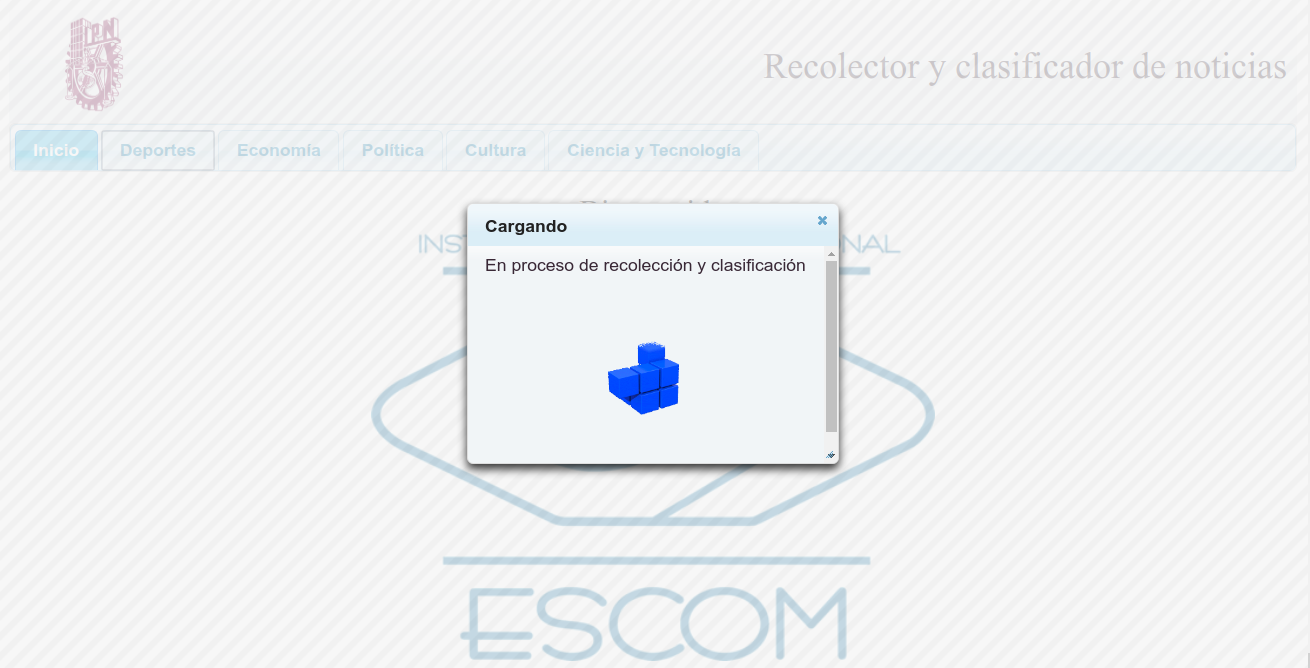
\includegraphics[scale=0.35]{imagenes/mensajeEspera.png}
\caption{Mensaje de espera}
\label{fig:loading}
\end{figure}


\subsection{Recolectar}


Esta etapa genera un subproceso el cual activa un script (desarrollado en \textbf{Python 3}) el cual activa la recolección de noticias en los sitio web definidos previamente, la información que se obtiene de cada artículo es la siguiente:

\begin{itemize}
	\item \textbf{URL de la noticia}
	\item \textbf{Título}
	\item \textbf{Fecha}
	\item \textbf{Autor}
	\item \textbf{Descripción} (Existen sitios web, donde las noticias no cuentan con una descripción)
	\item \textbf{Noticia}
\end{itemize}

La extracción de las noticias se hace en la página principal de los sitios web. Cabe destacar que en el proceso de recolección se valida que las noticias contengan al menos 180 palabras (en la redacción de \textbf{Noticia}), de lo contrario no se extrae. Ademas se ha definido un tiempo máximo de espera en esta etapa, el cual es de 30 segundos, después de concluir el periodo y haber recolectado la información, se procede con la etapa de \textbf{Clasificación}, de lo contrario si no se recolecto ninguna noticia se muestra el mensaje \textbf{Se ha agotado el tiempo de espera, no se han encontrado noticias, intentar mas tarde} (como se visualiza en la Figura \ref{fig:notNoRec}) y se detiene el proceso.

\begin{figure}[H]
\centering
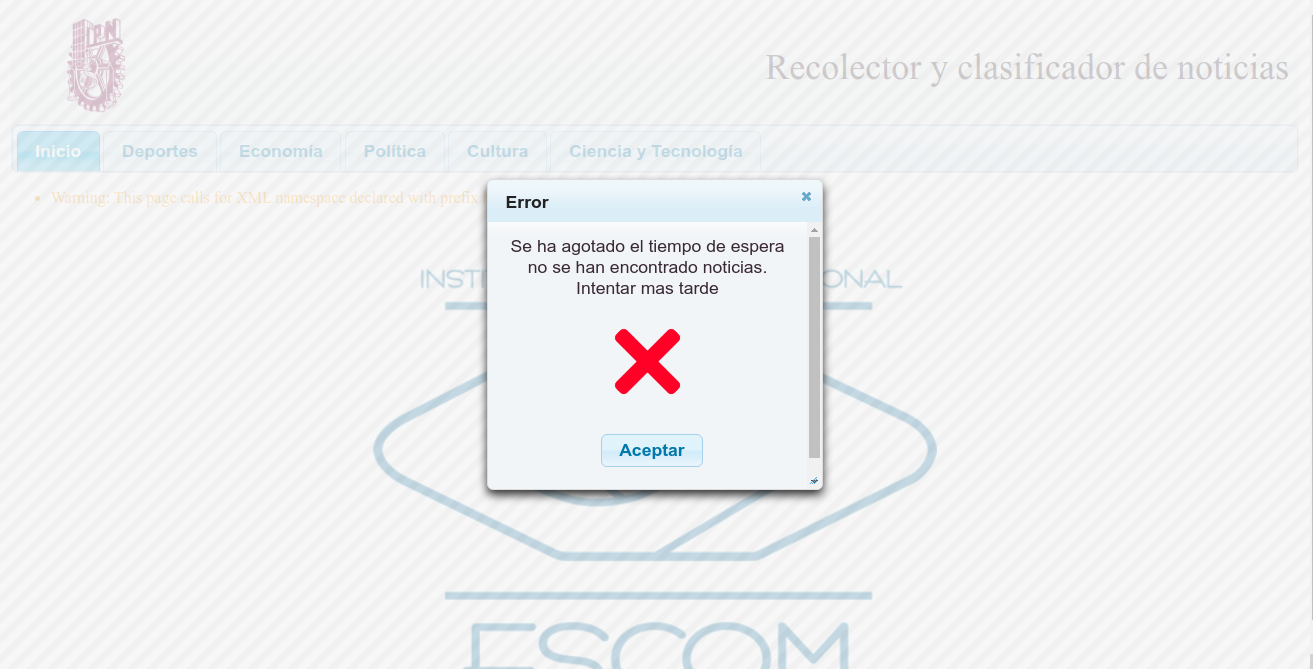
\includegraphics[scale=0.3]{imagenes/errorConectividad.png}
\caption{Mensaje de error en la recolección}
\label{fig:notNoRec}
\end{figure}

\subsection{Clasificar}

Después de recolectar las noticias se inicia la etapa de clasificación, el cual esta conformado por 5 tareas (como se muestra en la Figura \ref{fig:cp5:clasificacion}). Esta etapa genera un subproceso para ejecutar un script desarrollado en \textbf{Python 3}, el cual está encargado de llevar acabo cada tarea de esta sección. Cabe destacar que el proceso de clasificación solo utiliza el contenido de la noticia, los demás datos no son necesarios en esta etapa. A continuación se explica cada subtarea.

\begin{figure}[H]
\centering
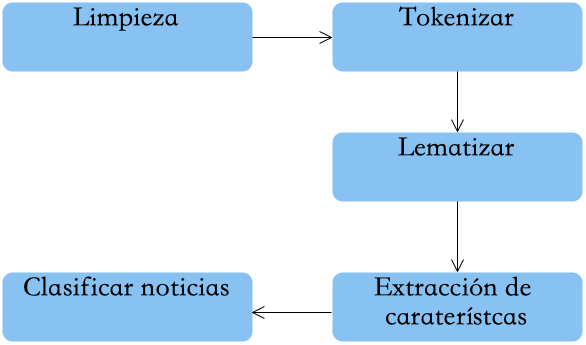
\includegraphics[scale=0.5]{imagenes/PreprocesamientoWeb.png}
\caption{Proceso de clasificación}
\label{fig:cp5:clasificacion}
\end{figure}

\begin{enumerate}

	\item \textbf{Limpieza}: En la sección de \textbf{Entrenamiento} el proceso de limpieza consiste en eliminar texto que no brinda información útil como, hipertexto, símbolos especiales (como \# $\dagger$ $\sqrt{ }$), \textit{emojis} (como \dSmiley \dCooley \dNinja), sin embargo en esta etapa no es necesario hacer esta limpieza, debido a que el vocabulario definido no contiene estos datos, por esta razón estos símbolos son ignorados en la extracción de características. Cabe señalar que lo único que es eliminado son los saltos de línea

	\item \textbf{Tokenizar}: Consiste en separar el texto en sus elementos mínimos por un espacio 

	\item \textbf{Lematizar}: Proceso que reduce cada una de las palabras tokenizadas en lemas

	\item \textbf{Extracción de características}: Se extrae palabras (características) con base al vocabulario definido al final de la etapa de entrenamiento, para crear un espacio vectorial por cada noticia (esta es la representación que el algoritmo entiende). Cabe destacar que las características son extraídas de forma binaria

	\item \textbf{Clasificar}: Al final de la sección \textbf{Entrenamiento} se almacenó el modelo clasificador el cual esta basado en el algoritmo \textbf{Maquinas de soporte vectorial}. Esta tarea utiliza el clasificador el cual recibe como entrada los vectores de características(los cuales representan el contenido de cada artículo) y como salida brinda la clasificación del conjunto de noticias, y son almacenadas por sección en un archivo \textbf{CSV}

\end{enumerate}


\subsection{Mostrar resultados}

Esta etapa consiste en presentar el resultado del proceso de clasificación en la herramienta. Cuando este proceso ha concluido se muestra el mensaje \textbf{Noticias listas para ser mostradas}, donde el usuario tiene la opción de elegir visualizar las noticias o cancelar el flujo del sistema, como se muestra en la Figura \ref{fig:notClass}.

\begin{figure}[H]
\centering
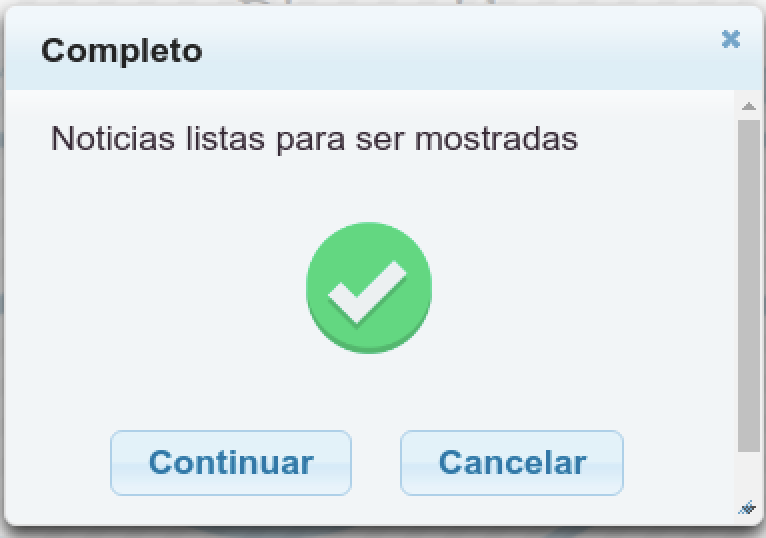
\includegraphics[scale=0.35]{imagenes/noticiasListasParaSerMostradas.png}
\caption{Mensaje que se muestra una vez clasificadas las noticias}
\label{fig:notClass}
\end{figure}

Si el usuario ha presionado la opción \textbf{Cancelar}, el proceso concluye y la herramienta muestra la Pantalla de Inicio (ver \ref{fig:PantallaInicio}), de lo contrario si se ha dado clic en \textbf{continuar}, se lleva acabo el proceso mostrado en la Figura \ref{fig:cp5:mostrar}, las tareas en color azul cielo siempre son llevadas acabo y las de color gris son opcionales. A continuación estas etapas son descritas.

\begin{figure}[H]
\centering
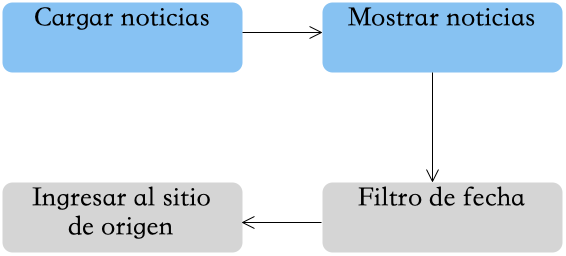
\includegraphics[scale=0.55]{imagenes/MostrarDatosApp.png}
\caption{Funcionalidad de la aplicación}
\label{fig:cp5:mostrar}
\end{figure}


\begin{enumerate}

	\item \textbf{Cargar noticias}: En el proceso de clasificación se crea un archivo \textbf{CSV} por cada sección con las noticias correspondientes, en esta etapa se obtiene los artículos de la sección elegida por el usuario

	\item \textbf{Mostrar noticias}: En la pantalla principal, las noticias se muestran por fecha de publicación, los datos mostrados por cada noticia son: \textbf{título de la noticia}, \textbf{resumen de la noticia}(de contar con ello), \textbf{autor} y finalmente la \textbf{fecha de publicación}. Como se muestra en la Figura \ref{fig:vistaNoticias}


	\item \textbf{Filtro fecha}: En la sección de las noticias, se muestra un menú con las opciones: \textbf{Hoy}, \textbf{Ayer}, \textbf{Dos días} y \textbf{Tres días o mas}. Este es una herramienta que permite filtrar los artículos por fecha de publicación. Por ejemplo, si el usuario desea visualizar noticias de un día anterior a la registrada por el sistema, se debe seleccionar la opción \textbf{Ayer}, en seguida la información de este periodo se muestra, como en la Figura \ref{fig:vistaNoticiasAyer}. Es importante mencionar que las noticias mostradas por defecto son las del día de consulta (\textbf{Hoy})

	\item \textbf{Ingresar al sitio de origen}: Cada noticia mostrada contiene la \textbf{URL} al sitio de origen de la noticia, si el usuario desea leer el artículo completo se debe dar clic en la noticia y la aplicación redirige el buscador a la pagina fuente

\end{enumerate}


\begin{figure}[H]
\centering
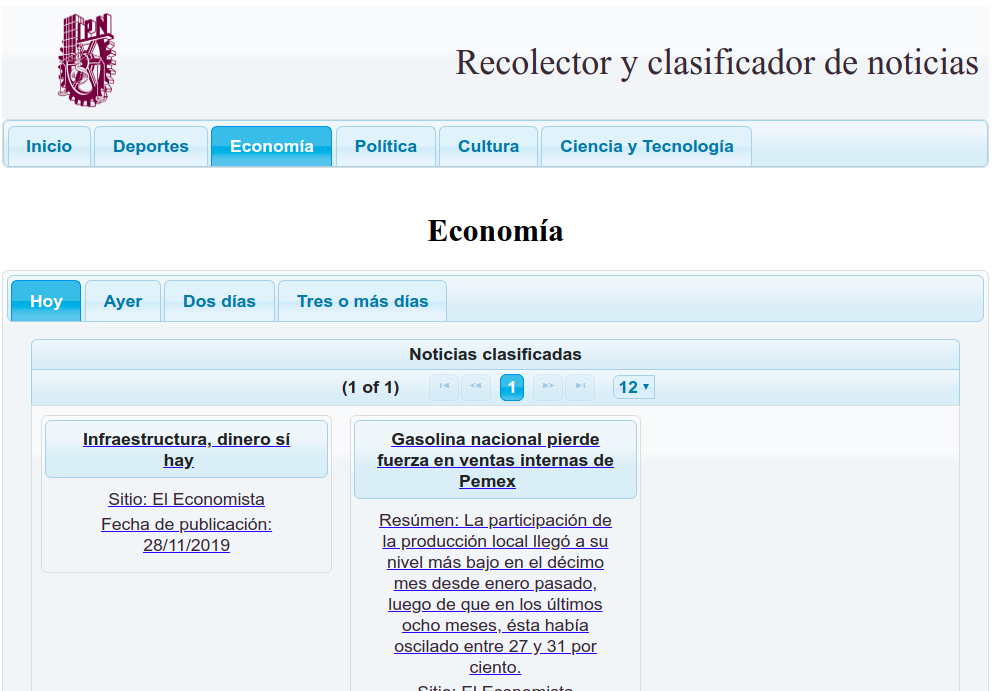
\includegraphics[scale=0.45]{imagenes/noticiasDeHoy.png}
\caption{Vista de las noticias recolectadas}
\label{fig:vistaNoticias}
\end{figure}




\begin{figure}[H]
\centering
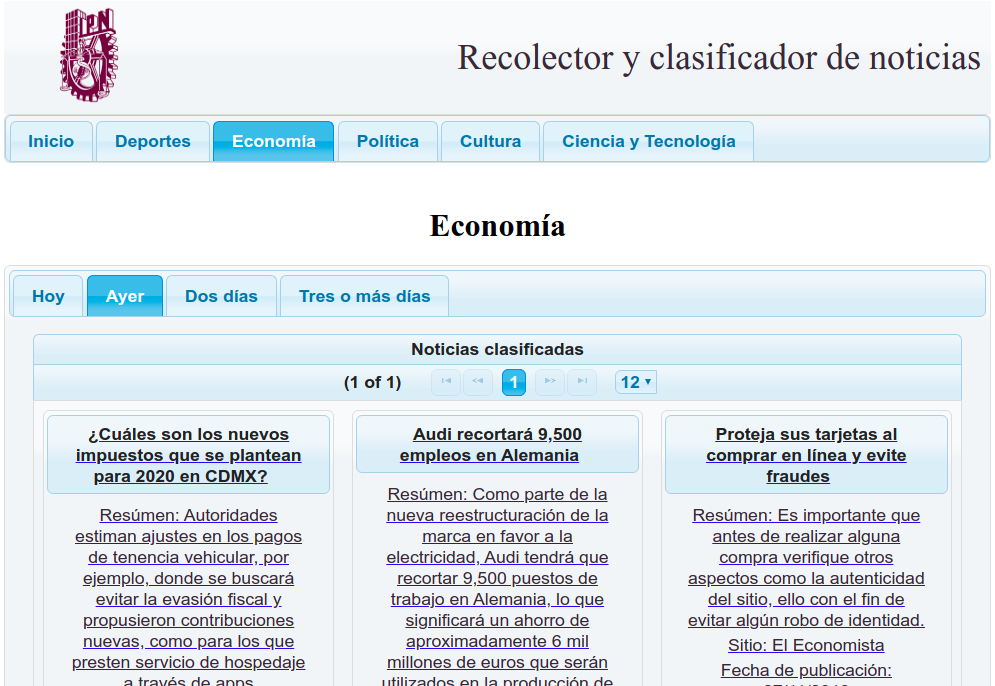
\includegraphics[scale=0.45]{imagenes/noticiasDeAyer.png}
\caption{Vista de las noticias recolectadas del día de ayer}
\label{fig:vistaNoticiasAyer}
\end{figure}


\end{document}